\documentclass[conference]{IEEEtran}
\IEEEoverridecommandlockouts
% The preceding line is only needed to identify funding in the first footnote. If that is unneeded, please comment it out.
\usepackage{cite}
\usepackage{amsmath,amssymb,amsfonts}
\usepackage{algorithmic}
\usepackage{graphicx}
\usepackage{textcomp}
\usepackage{xcolor}
\usepackage[export]{adjustbox}
\usepackage[utf8]{inputenc}
\def\BibTeX{{\rm B\kern-.05em{\sc i\kern-.025em b}\kern-.08em
    T\kern-.1667em\lower.7ex\hbox{E}\kern-.125emX}}

\begin{document}

\title{Práctica final: Competición de mini-sumo\\
%\thanks{Identify applicable funding agency here. If none, delete this.}
}

\author{
    \IEEEauthorblockN{
        %\large{Andrés Casasola Domínguez}\\
        %\large{Juan Manuel Vázquez Jiménez}\\
        \large{Andrés Casasola Domínguez}\\
        \large{Juan Manuel Vázquez Jiménez}\\
    }
    \IEEEauthorblockA{
        \textit{\large{Asignatura: Microbótica}}\\       
        \textit{\large{Febrero 2020}}\\
    }
}

\maketitle

\section{\large{Resumen}}
\large{En este proyecto se va a desarrollar un robot de dos ruedas para competir en luchas de mini-sumo. En la figura \ref{fig:robot}, se puede ver una imagen del robot.}


\begin{figure}[h]
    \centering
    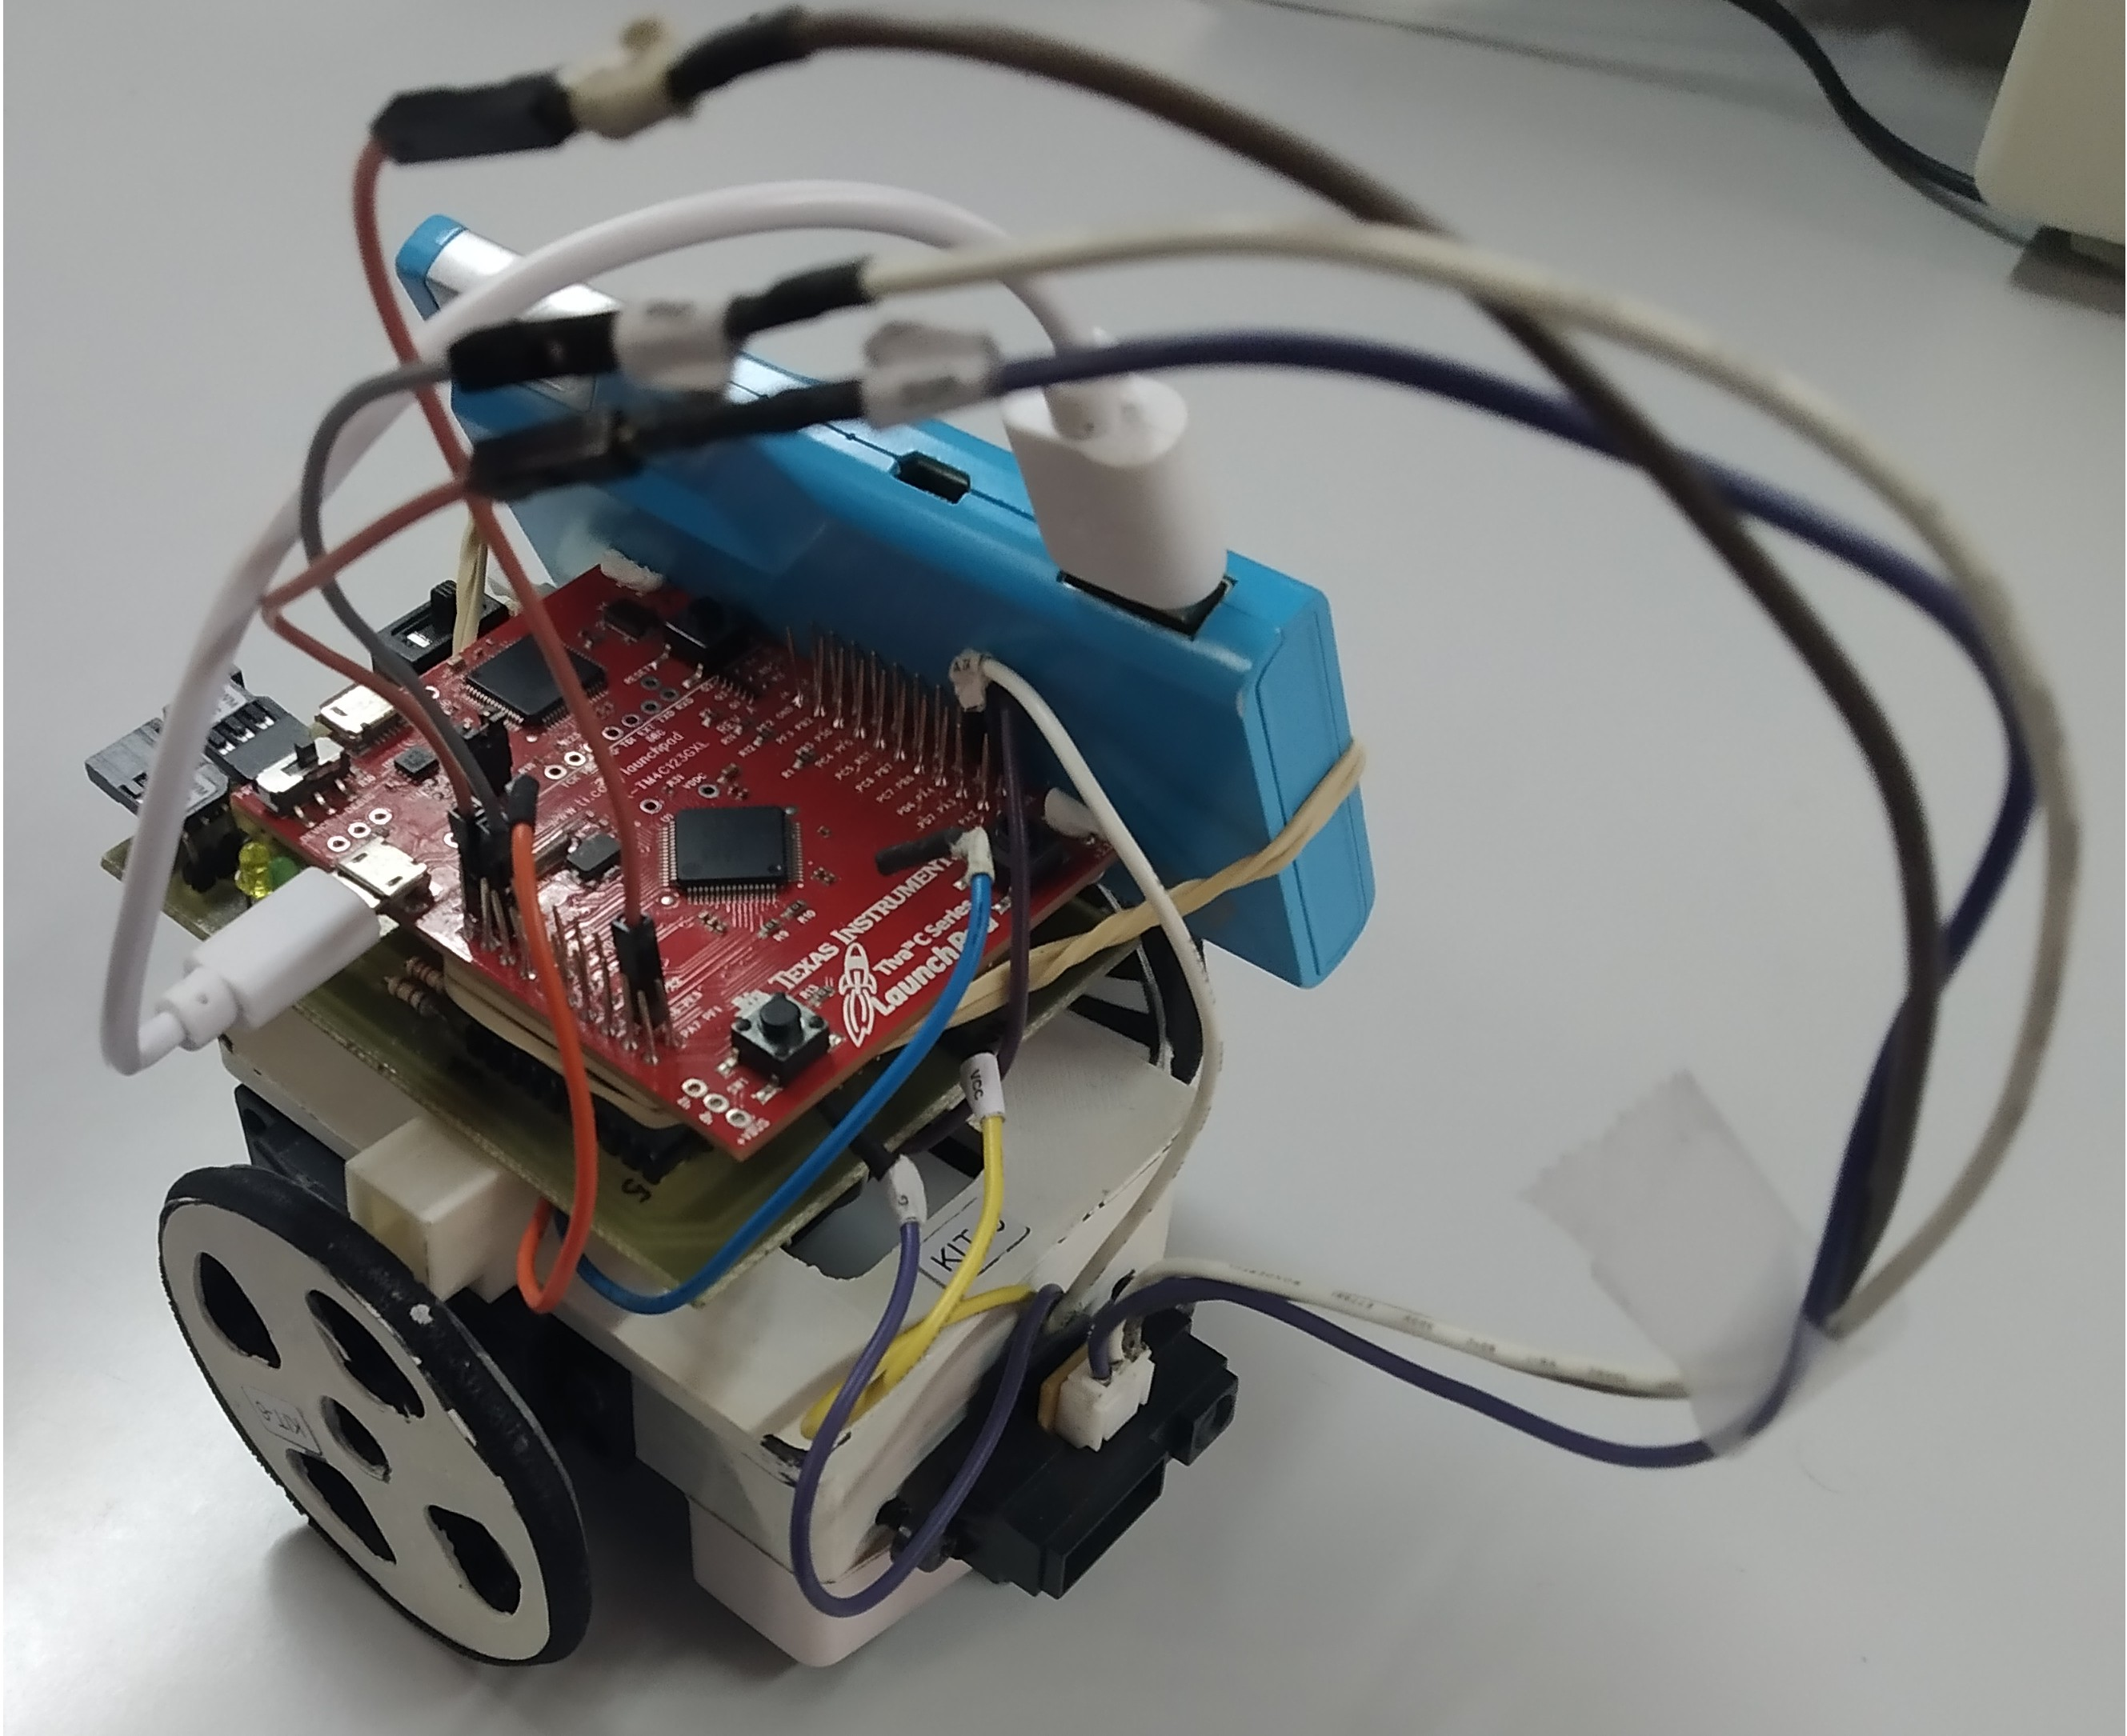
\includegraphics[width=0.9\linewidth, frame]{photos/microbot1_cut2.jpg}
    \caption{\large{Imagen del robot montado}}
    \label{fig:robot}
\end{figure}

\section{\large{Caracteristicas}}
\large{El robot utiliza dos sensores para moverse por la pista sin salirse, detectando obstáculos y reaccionando ante ellos. El sensor que detecta cuando se esta saliendo de pista, es un encoder y el que detecta obstáculos, es el sensor de distancia \textit{Sharp GP2Y0A41SK0F}. Además, el robot tiene una batería acoplada en el lateral con masilla moldeable y un par de elásticos. Tanto el encoder como el sensor de distancia estan posicionados en la cara frontal del robot, por lo tanto, el robot siempre se desplazará hacia delante.}\\

\section{\large{Jerarquia de ficheros}}
Para la implementación se han creado librerías que abstraen el codigo main del bajo nivel de los timers para el PWM o para el ADC, por ejemplo. De esta forma, mediante el uso de algunas funciones sencillas e intuitivas, se puede cambiar el estado de movimiento y sensado del robot. En la figura \ref{fig:jerarquia} se puede ver un diagrama en el que se representa la jerarquía de ficheros.

\begin{figure}[h]
    \centering
    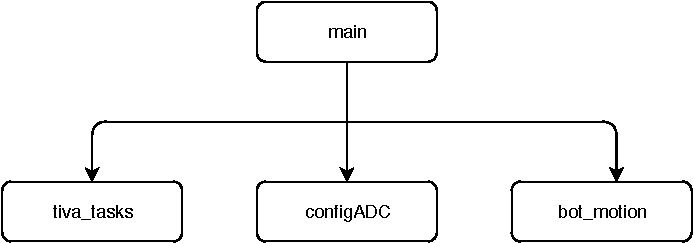
\includegraphics[width=\linewidth]{photos/jerarquia.pdf}
    \caption{\large{Jerarquía de los ficheros mas representativos en el proyecto.}}
    \label{fig:jerarquia}
\end{figure}

\section{\large{Comportamiento}}
El comportamiento del robot es puramente reactivo, es decir, el robot siempre se desplazá hacia delante a la espera de eventos, cuando detecta que se sale de pista, realiza un giro de 180 grados, cuando detecta un obstáculo realiza una maniobra de flanqueo para posicionarse detras del obstáculo y continua hacia delante. Si el robot comienza una maniobra de flanqueo y detecta que se sale de pista, aborta la maniobra y realiza un giro de 180 grados.\\

La traducción en cuanto al funcionamiento del sistema consiste en una espera continua de interrupciones. Las fuentes de interrupciones pueden ser o un flanco en el sensor encoder o un dato proveniente del ADC. Cada interrupción es tratada por una tarea, por tanto, existen dos tareas, una para procesar los cambios en el encoder y otra para procesar los datos del ADC. Es importante aclarar que la tarea del encoder activa o bloquea la tarea del sensor, de esta forma, no salirse de pista es siempre el objetivo prioritario.

\section{\large{Especificaciones}}
Las especificaciones cumplidas por este diseno son de nivel 1, comportamiento reactivo.

\section{\large{Diagramas de flujo del codigo}}
En la figura \ref{fig:main}, se puede ver el diagrama de flujo del fichero principal, \textit{main.c}.\\

En la figura \ref{fig:config}, se puede ver la función de configuración, \textit{config()}.\\

En la figura \ref{fig:reactive}, se puede ver la tarea del encoder de mayor prioridad, \textit{ReactiveTask()}.\\

En la figura \ref{fig:sensor}, se puede ver la tarea del ADC de menor prioridad, \textit{SensorTask()}.\\

\begin{figure}[h]
    \centering
    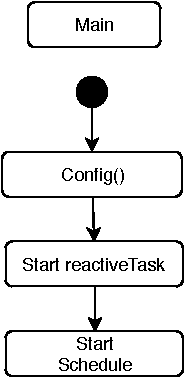
\includegraphics[width=0.4\linewidth]{photos/main.pdf}
    \caption{\large{Diagrama de flujo del fichero \textit{main.c}.}}
    \label{fig:main}
\end{figure}

\begin{figure}[h]
    \centering
    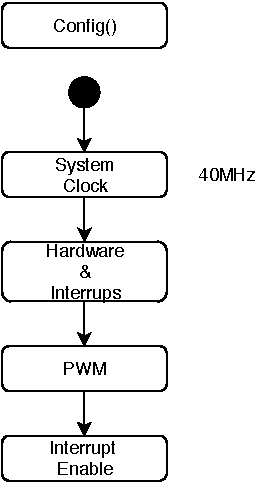
\includegraphics[width=0.55\linewidth]{photos/config.pdf}
    \caption{\large{Diagrama de flujo de la función de configuración \textit{config()}.}}
    \label{fig:config}
\end{figure}

\begin{figure}[h]
    \centering
    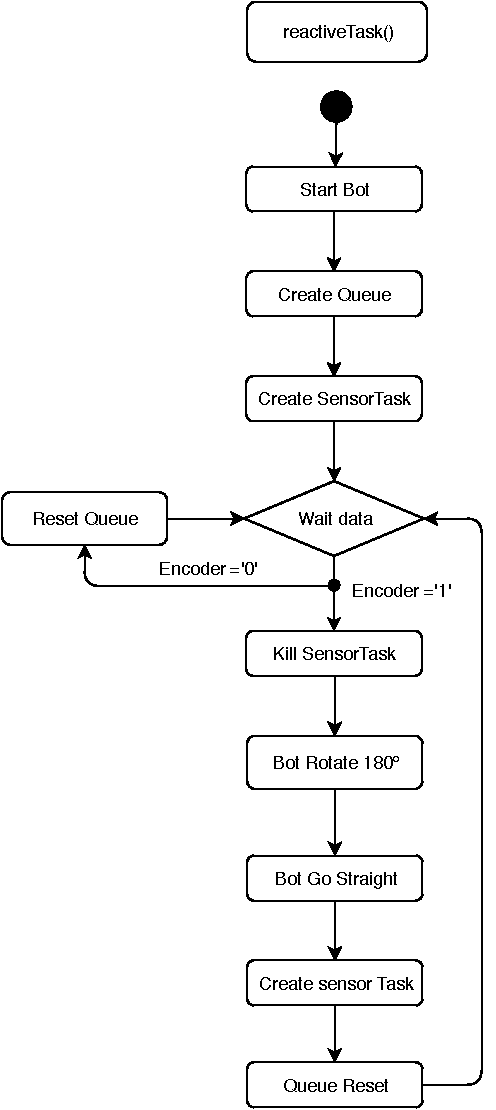
\includegraphics[width=\linewidth]{photos/reactive.pdf}
    \caption{\large{Diagrama de flujo de la tarea \textit{ReactiveTask()}.}}
    \label{fig:reactive}
\end{figure}

\begin{figure}[h]
    \centering
    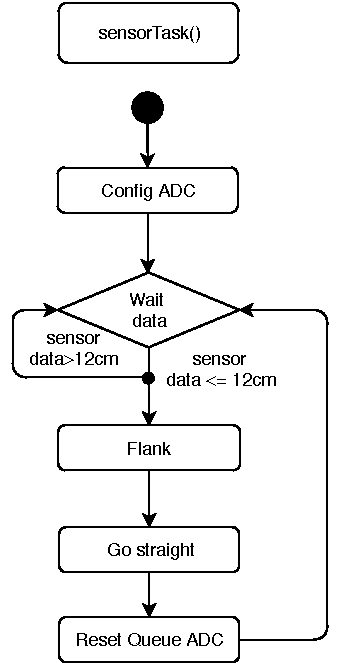
\includegraphics[width=0.7\linewidth]{photos/sensorTask.pdf}
    \caption{\large{Diagrama de flujo de la tarea \textit{SensorTask()}.}}
    \label{fig:sensor}
\end{figure}

\end{document}

